In conclusion, the higher the fretting position, the more intonation error there is. The relationship is not a linear one but quite complicated and can be modelled with the equation (\ref{eqn39}). By plotting the collected data and performing the goodness-of-fit test, it confirms the validity of the equation. \par
By choosing a simplified model of the guitar, it makes the calculations easier and creates a useful approximation model. However, the model doesn't take into account several factors in reality that can affect the intonation. For example, the use of a capo to simulate the fretting action of a human finger. The contact surface of a human finger on the string is very small, but that of a capo is much bigger. This can lead to more deformation of the string when using the capo and consequently an increase in tension \& frequency. Also, when fretting down on the string we don't normally press down directly on the fret like the capo, but a bit behind. This can depress the string more and lead to a higher intonation error. Another factor is the guitar neck isn't always rigid and straight like in the model but sometimes slightly bowed, either from the tension of the strings or set up by the player, which can also affect the intonation. An assumption I made in the experiment is the point of pressing down on the string would have no friction, therefore the tension increase would be distributed evenly throughout the string, but in reality the finger or the capo would have a small amount of friction that can affect the result. Another limitation of the model is it only applies to plain unwound steel strings, so it can only be used for the highest 3 strings on a guitar, but for the other 3 wound strings we would need a different model.\par

An observation I can make from equation (\ref{eqn39}) is that it is not dependent on the gauge (thickness) of the string I use. However, this conflicts with my experience, because when playing I would notice the thicker G string would exhibit more intonation shift than the thinner high E string. To investigate this, I repeat the experiment with my thinner B string and E string, tuning them to their standard frequencies ($B_3: 246.94$Hz and $E_4: 329.63$Hz). The collected and processed data for these are in the Appendix.

\begin{figure}[!htb]
    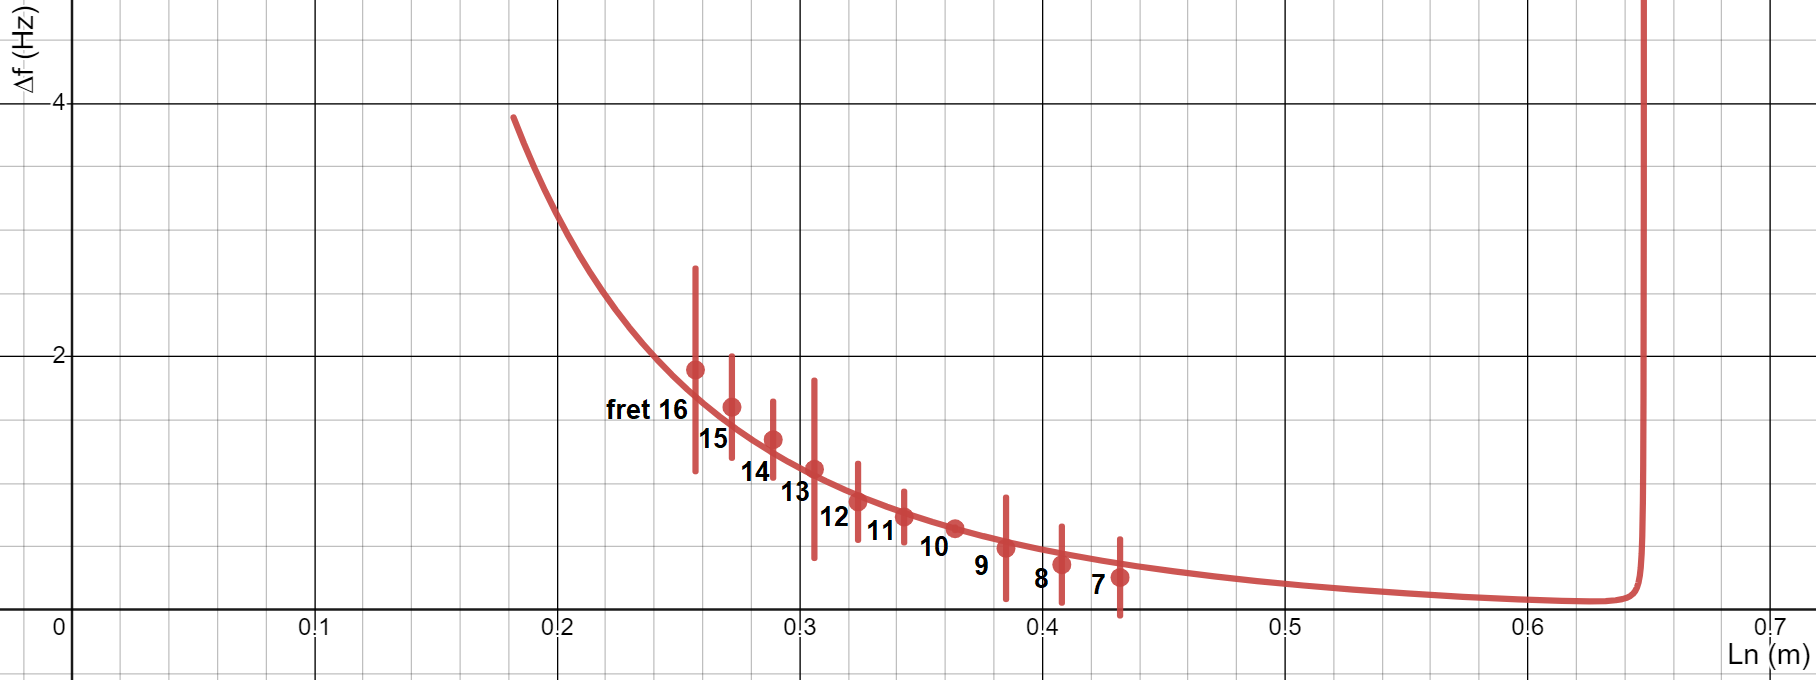
\includegraphics[width = \textwidth]{ee/compare b string.png}
    \caption{Curve for B string with data points and error bars} \label{fig10}
\end{figure}
\begin{figure}[!htb]
    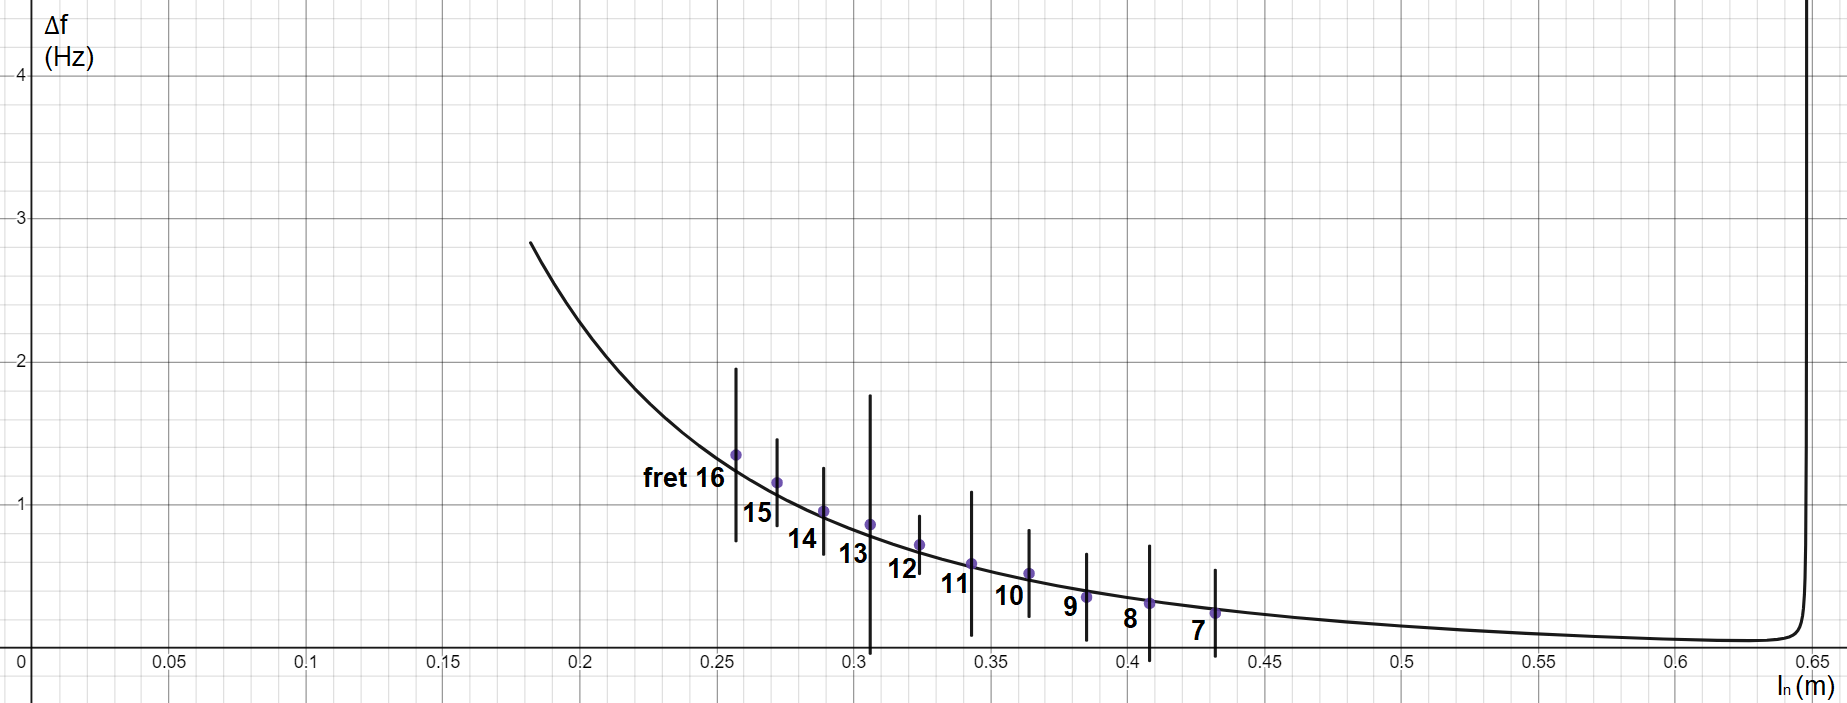
\includegraphics[width = \textwidth]{ee/compare e string.png}
    \caption{Curve for E string with data points and error bars} \label{fig11}
\end{figure}
\begin{figure}[!htb]
    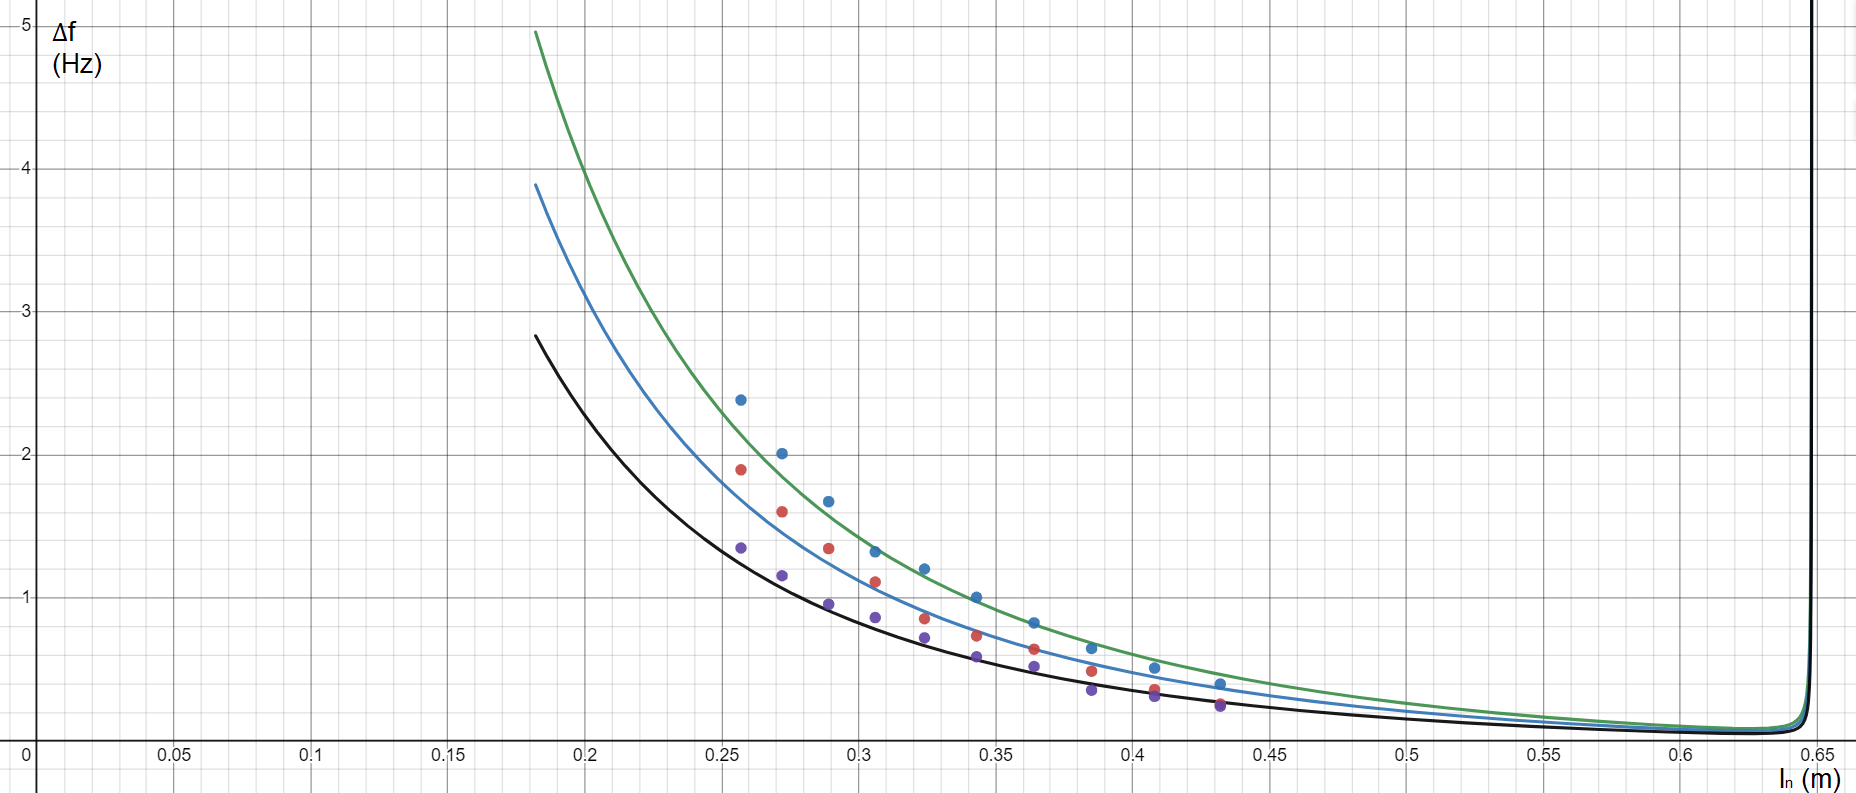
\includegraphics[width = \textwidth]{ee/all 3.png}
    \caption{Curve for all 3 strings with data points, error bars have been hidden for clarity} \label{fig6}
\end{figure}
Overall we see that the graphs of B and E strings are successively lower, meaning the intonation deviation on those strings are less, showing that my observation is correct. I believe this is because the strings have different $f_0$ which contribute to the differences in the curves. We can also make some observations from the data. Most noticeably, data points for higher frets are slightly higher than predicted by the curve. This is the same trend observed with the original data of the G string, and I believe the cause is the same: the capo not fretting directly down on the string but slightly pushing the string sideways. Also, we can see the error bars generally gets larger for the thinner strings (error bars for E string are generally bigger than B string, and error bars for B string are also bigger than G string). This means there is an increase in variance of the frequency for trials at each fret position for thinner strings. This might be because thin strings might slip slightly sideways under the capo each time it's plucked, meaning for the same fret, there will be a slightly different frequency for each pick, even though the capo is never moved. It is also noticeable that there is a large error bar at fret 13 and 16 for the B and E strings. Upon closer inspection of the guitar, it seems like the fret at these positions are quite worn down. This might cause the string to slip more under the capo, explaining the large error bar. Some improvements I can suggest for the experiment is to use a stronger capo to minimize slipping, level the guitar frets before carrying out the experiment, and try to pluck gently to avoid pushing the string sideways too much.

Therefore, overall in order to minimize intonation error, it is recommended to use thinner gauge strings. However, players need to take into account other factors as well when changing strings. For example, it's not recommended for players with a slightly heavier playing style, because the lower resistance of thinner strings will make it more likely to be pushed sideways when fretted rather than directly down on the fret, which will also cause intonation shifts.\par

From the graph of the equation relating $\Delta f$ and $l_n$ we can also evaluate the effects of changing other variables on the shape of the curve. It is impossible to have zero intonation deviation through the whole graph, but I can try ways to minimize this error. I notice the variable that has the most effect on the graph is $a$, the vertical distance between top of the bridge saddle and the frets. Simply reducing the value of $a$ by around 1 mm, bringing it from 3.3 mm down to 2 mm (\SI{2e-3}{m}) is enough to reduce the intonation shift at fret 16 down to around 1.8 Hz (Figure \ref{fig12}), which would be equivalent to $\frac{1.8}{C5-B4}\cdot 100 = \frac{1.8}{523.25-493.88} \cdot 100 \approx 6$ cents, which is almost unnoticeable to the human ear. \cite{loeffler}

\begin{figure}[!h]
    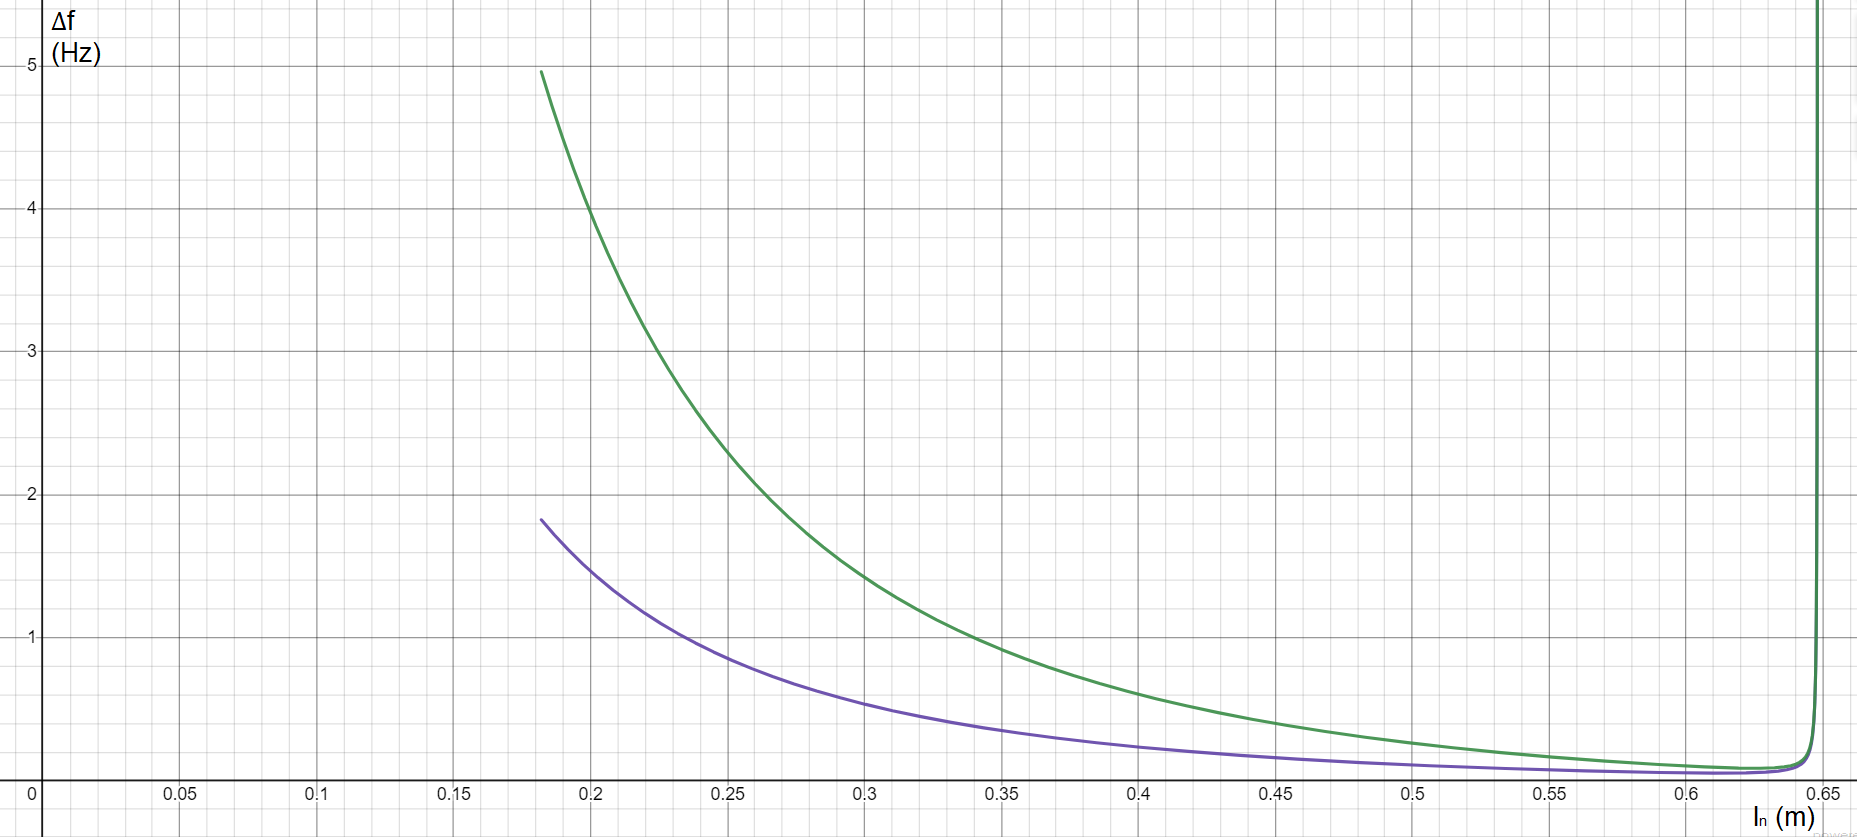
\includegraphics[width = \textwidth]{./ee/compare_graph_a.png}
    \caption{Comparing before (green) and after changing value of $a$ (purple)} \label{fig12}
\end{figure}
So a lower string action would be better for intonation. Guitar manufacturers as well as guitarists can take this into account when setting up their guitars to reduce the intonation error. However, reducing the saddle height too much will cause buzzing of the string, where the string hit against other frets when it is plucked and vibrating. This will reduce the quality of the tone and might even lead to more intonation error. Therefore, a careful trial and error approach is needed when adjusting for a good intonation. \par
Overall from the investigation we see that the intonation of a guitar string is a complicated variable and is affected by a lot of different factors. We cannot eliminate it completely, but there are some things we can do to control it to try and minimize the intonation shifts, such as using low gauge strings and having a low action.